% Possible values for aspect ratio are: 169, 1610, 149, 54, 43 and 32.
\documentclass[aspectratio=1610]{beamer}
\usetheme{cern}

% Change bullet points
\usepackage{enumitem}
\setbeamertemplate{itemize items}[square]
\setitemize{label=\raisebox{0.3ex}{\usebeamerfont*{itemize item}
\usebeamercolor[fg]{itemize item}
\usebeamertemplate{itemize item}}}
%\setlist[itemize]{leftmargin=*, itemsep=0pt, parsep=2pt, labelsep*=2em, labelindent=0em, before=\vspace{-\dimexpr\baselineskip +2.6\partopsep}}

% CERN blue is Pantone 286 = RGB 56 97 170, defined as cern@blue below
\definecolor{cern@ltblue}{rgb}{0.415686,0.611765,0.964706} % RGB 106 156 246
\definecolor{cern@blue}  {rgb}{0.219608,0.380392,0.666667} % RGB  56  97 170
\definecolor{cern@dkblue}{rgb}{0.082353,0.184314,0.364706} % RGB  21  47  93

% Complimentary colours
\definecolor{cern@ltcomp}{rgb}{0.666667,0.525490,0.219608} % RGB 170 134  56
\definecolor{cern@dkcomp}{rgb}{0.364706,0.266667,0.047059} % RGB  93  68  12

%\setbeamercolor{title}               {bg=cern@blue,fg=white}
%\setbeamercolor{frametitle}          {bg=cern@blue,fg=white}
%\setbeamercolor{section in head/foot}{bg=cern@ltblue,fg=white}
\setbeamercolor{itemize item}         {fg=cern@dkcomp}
\setbeamerfont{itemize item}          {size=\large}



%%
%% Get packages that we need
%%

% Adjust page margins on-the-fly
\usepackage{changepage}

% Change fonts to Avenir
% Note: need to compile with xelatex to use this package
\usepackage{fontspec}
\setsansfont{AvenirLTStd-Book}

\usepackage[showboxes,overlay,absolute]{textpos}
\usepackage[overlay,absolute]{textpos}
\setlength{\TPHorizModule}{.01\paperwidth} % Horizontal units are percent of paper width
\setlength{\TPVertModule}{.01\paperwidth}  % Make vertical units equal to horizontal units
\textblockorigin{.5\paperwidth}{4.25ex}

% Headings within slides
\usepackage{xcolor}
\usepackage{tabularx}



%%
%% Title page
%%

\author{\Large Dr. Michael Davis for the CTA Team}
\title[CTA in Production (ATLAS)]{CERN Tape Archive (CTA) in Production :\\
ATLAS migration report and next steps\\}
\date{28 June 2020}

% The ATLAS experiment is migrating from CASTOR to CTA during the week of 22 June. This marks the end
% of the CASTOR ATLAS service and the first production instance of CTA. The CTA Team will give a report
% on the migration of ATLAS and a status update on the migration of the other experiments.

\begin{document}

\frame{\titlepage}

\begin{frame}{EOS+CTA in Production ``by end 1Q 2020''}
   \centering
   
\includegraphics[width=\textwidth]{images/CASTOR_EOS+CTA_Logo}
\end{frame}

\begin{frame}{ATLAS Migration Plan}
\begin{columns}
	\begin{column}{0.4\textwidth}
		\begin{center}
         \includegraphics[width=\textwidth]{images/CTA_Deployment_Atlas}
		\end{center}
	\end{column}
	\begin{column}{0.55\textwidth}
   \begin{itemize}
      \item Commissioning tests
      \item Disable CASTOR ATLAS
      \item Migrate metadata from CASTOR to CTA
      \item Put EOS+CTA ATLAS into production
   \end{itemize}
	\end{column}
\end{columns}
\end{frame}

\begin{frame}{ATLAS Reprocessing Campaign}{}
% On Tue 21st Atlas started a major reprocessing campaign, scheduled to recall 4PB of data from a
% production instance of CTA. The service has performed well so far, reaching sustained throughput of
% 5GB/s, limited in this case by the network interfaces of the CTA nodes. More nodes will be added in
% order to demonstrate the horizontal scaling of the service.
   \centering
   \vspace{1ex}
   {\LARGE\color{cern@blue}January: Recall of Data18\\
   February: Recall of Data17}

\begin{adjustwidth}{-1cm}{-1cm}
   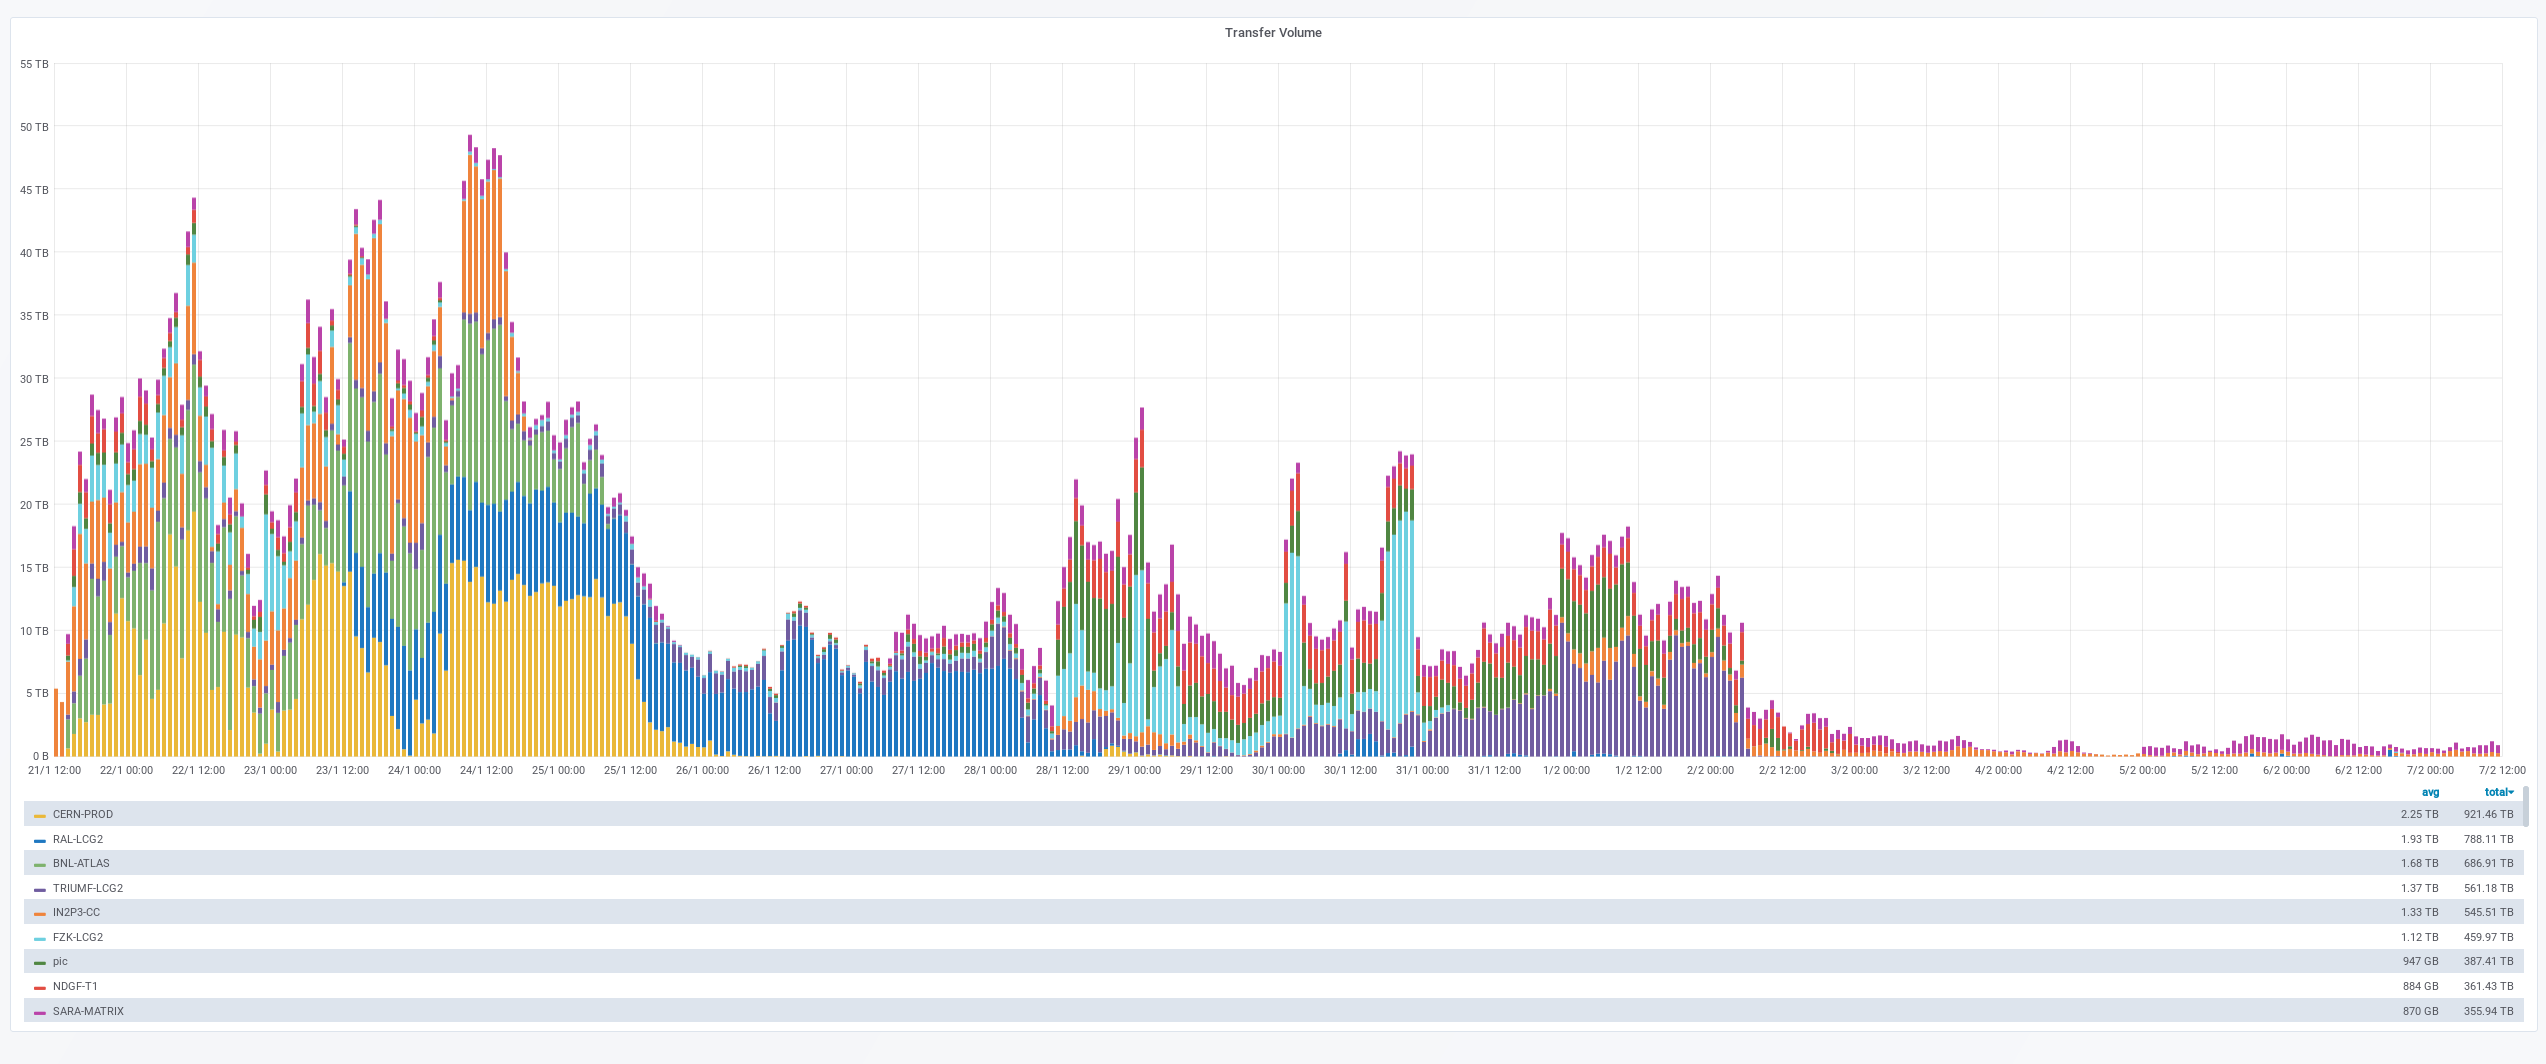
\includegraphics[width=\linewidth]{images/RecallTest}
\end{adjustwidth}
\end{frame}

\begin{frame}{ATLAS Data Carousel/Rucio WS Report}{}
   \begin{itemize}
      \item 5 PB recalled @ 4--5 GB/s %(Limiting factor was hardware and network bandwidth)
      %\item Software scaled smoothly as more hardware was added
      %\item Very efficient tape recall (80\% tape drive efficiency for Enterprise drives)
      \item CTA was the fastest site
      \item CTA had the lowest site error rate (< 350 errors)
      \item \textbf{CTA demonstrated to be performant and reliable for large volume transfers}
      \item No need for further recall tests: CTA did not participate in data16 and data15 recalls
   \end{itemize}
\end{frame}

\begin{frame}{March/April : SFO Integration Tests}{}
   \begin{center}
      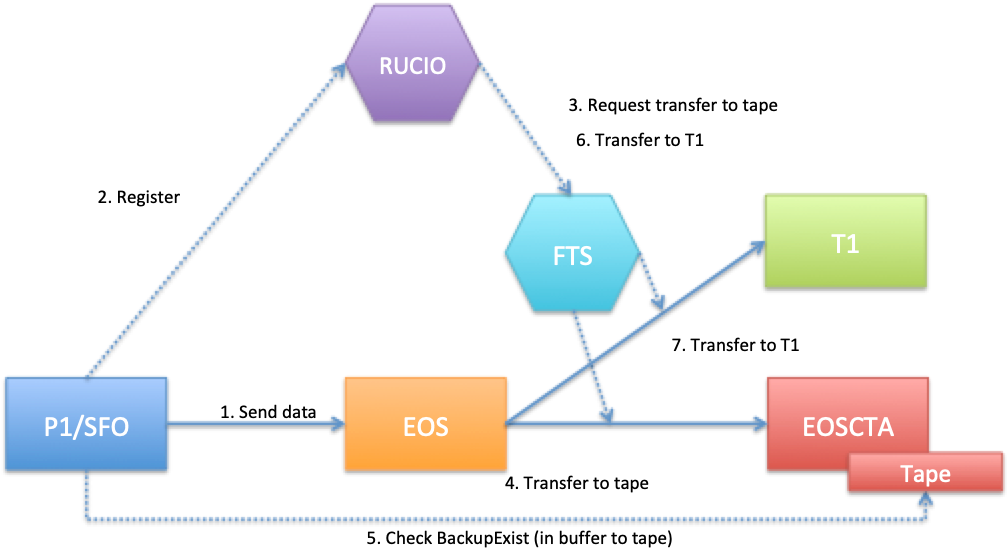
\includegraphics[width=0.5\linewidth]{images/SFO_test_setup}
   \end{center}
      {\normalsize
      \begin{itemize}
         \item ``File safely on tape'' check caused a high rate of metadata queries to EOS
         \item Problem will be fixed using FTS
         \item In the interim, ATLAS implemented a local metadata cache to reduce the number of
            queries to an acceptable rate
      \end{itemize}}
\end{frame}

\begin{frame}{June : ATLAS Migration}
   \normalsize
   \textbf{28 May}
   \begin{itemize}
      \item Re-test SFO integration
   \end{itemize}
   \textbf{15 June}
   \begin{itemize}
      \item Disable writes to CASTOR ATLAS
      \item Consistency check between Rucio catalogue and CTA catalogue
   \end{itemize}
   \textbf{23 June}
   \begin{itemize}
      \item Permanently disable all access to CASTOR ATLAS
      \item Migrate metadata for 85 million files
   \end{itemize}
   \textbf{25 June}
   \begin{itemize}
      \item Migration complete
      \item Consistency check between CASTOR export and CTA import
   \end{itemize}
   \textbf{29 June}
   \begin{itemize}
      \item \textbf{EOS+CTA ATLAS in operation}
   \end{itemize}
\end{frame}

\begin{frame}{23--25 June : ATLAS Migration}
\begin{columns}
	\begin{column}{0.45\textwidth}
		\begin{center}
		  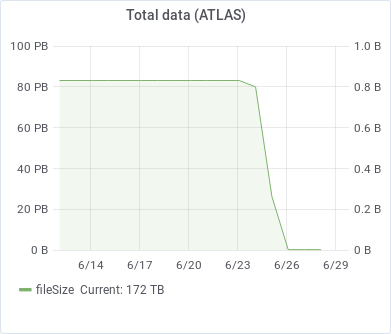
\includegraphics[width=\textwidth]{images/Migration_CASTOR}

        CASTOR
		\end{center}
	\end{column}
	\begin{column}{0.45\textwidth}
		\begin{center}
		  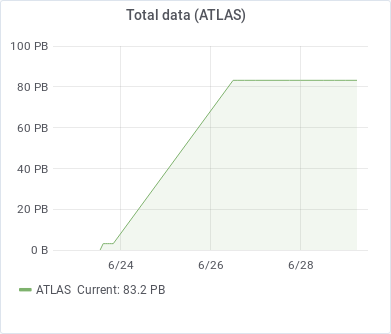
\includegraphics[width=\textwidth]{images/Migration_CTA}

        CTA
		\end{center}
	\end{column}
\end{columns}
\end{frame}

\begin{frame}{What's next for CTA? ALICE}
\begin{columns}
	\begin{column}{0.4\textwidth}
		\begin{center}
		  \includegraphics[width=\textwidth]{images/CTA_Deployment_ALICE}
		\end{center}
	\end{column}
	\begin{column}{0.55\textwidth}
		\begin{itemize}
        \item JAlien + EOS + CTA
		  \item SSD tape buffer + 5 PB HDD cache for retrieves
		  \item ALICE recall tests underway
        \item ALICE write tests in July
        \item Put into production after the summer
		\end{itemize}
	\end{column}
\end{columns}
\end{frame}

\begin{frame}{What's next for CTA? CMS and LHCb}
   \begin{itemize}
      \item Integration tests have started
   \end{itemize}
\begin{columns}
	\begin{column}{0.4\textwidth}
		\begin{center}
		  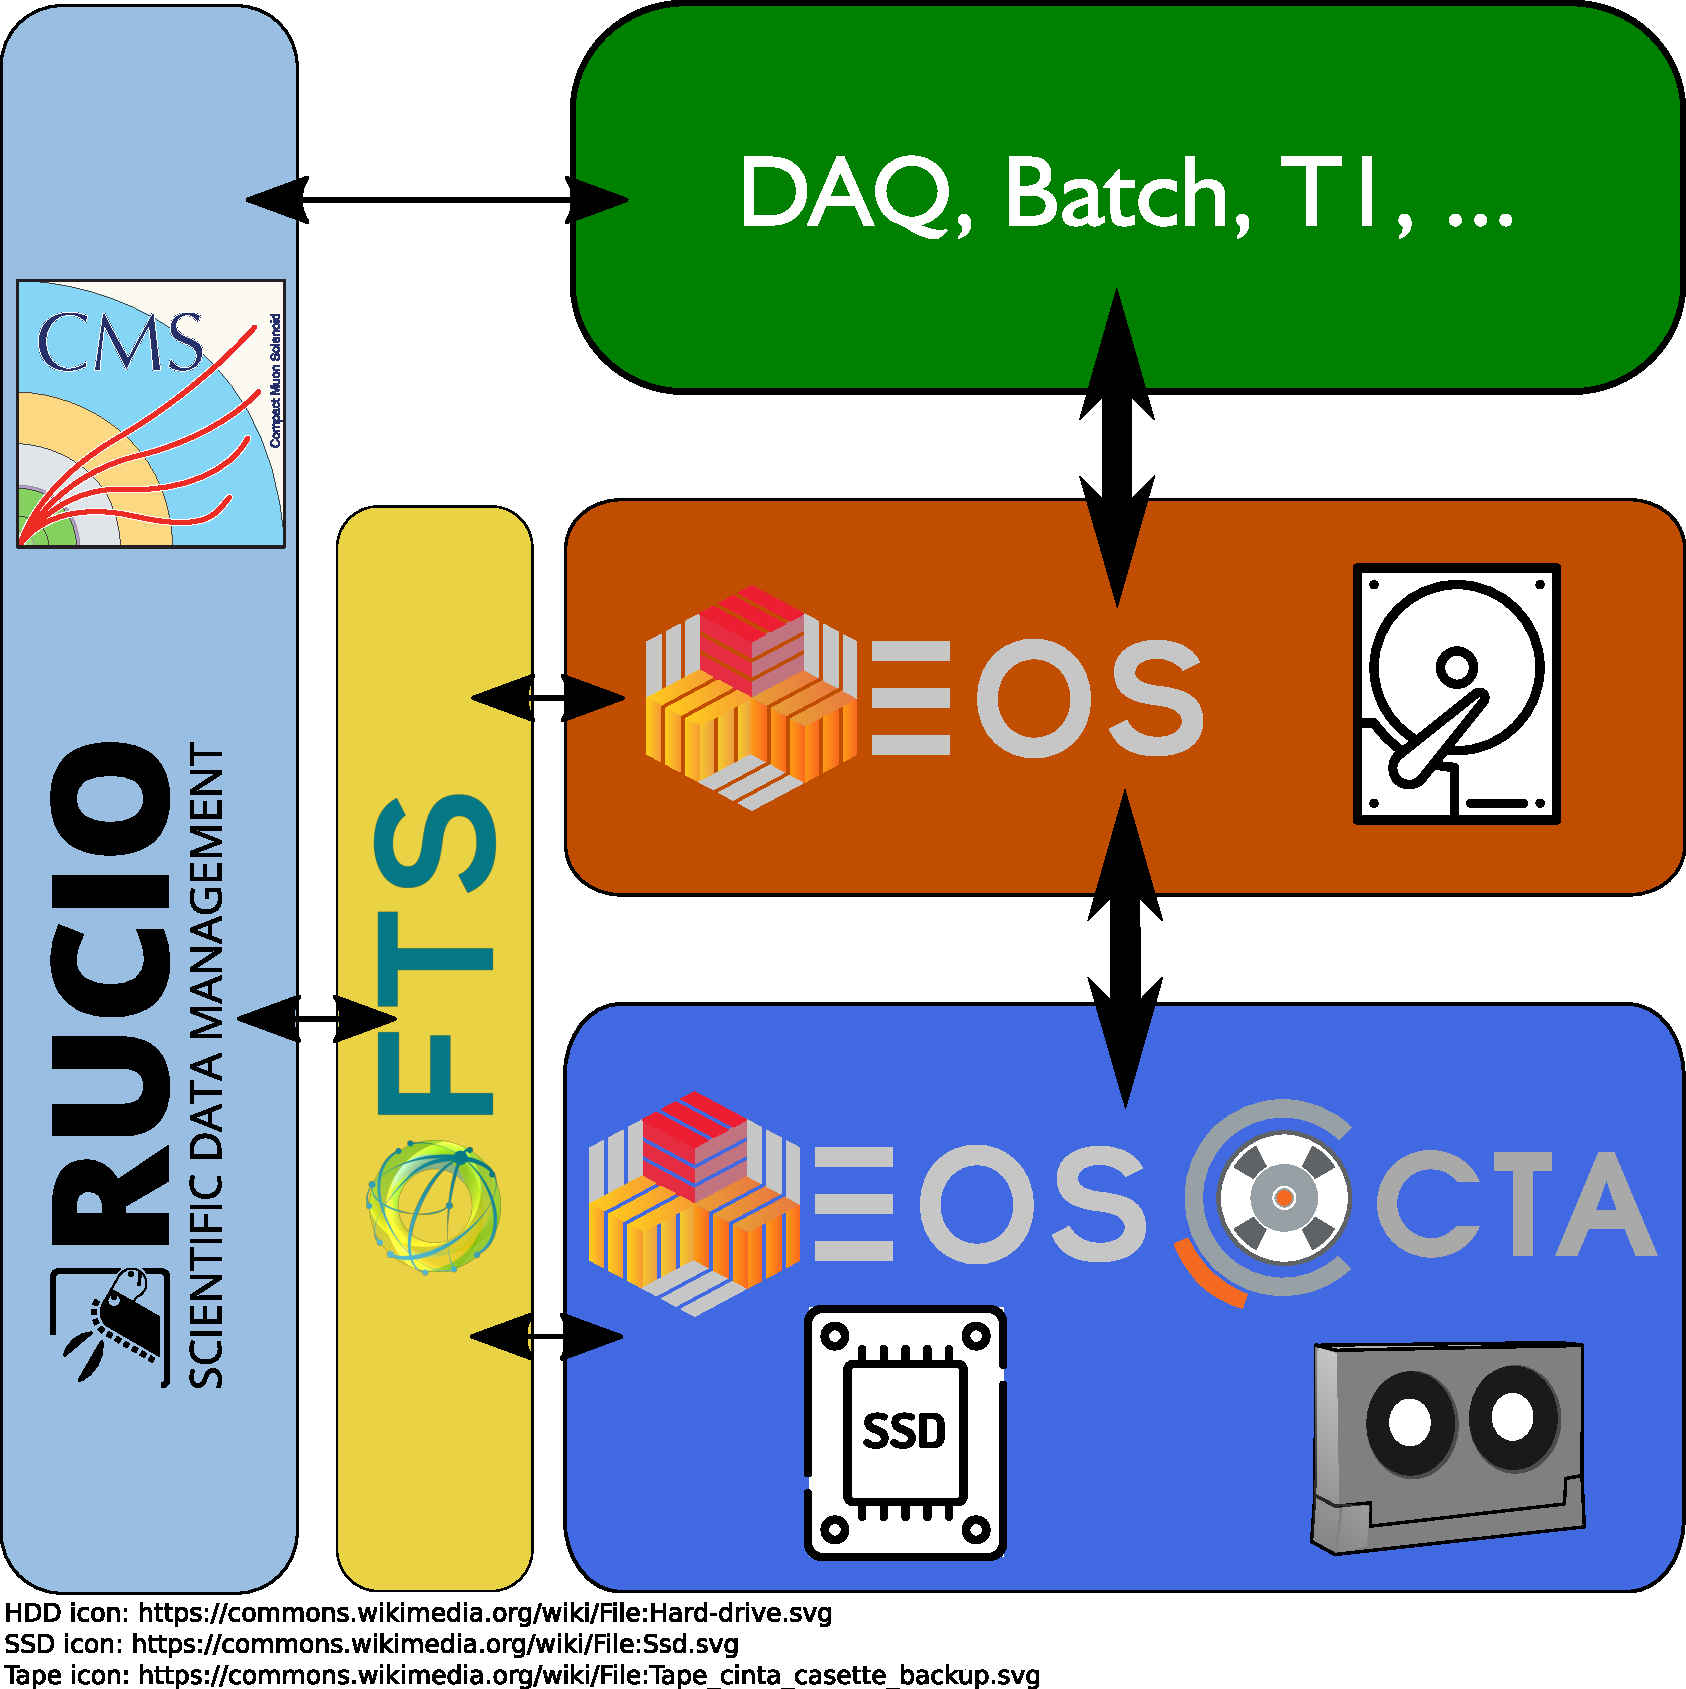
\includegraphics[width=\textwidth]{images/CTA_Deployment_CMS.pdf}
		\end{center}
	\end{column}
	\begin{column}{0.4\textwidth}
		\begin{center}
		  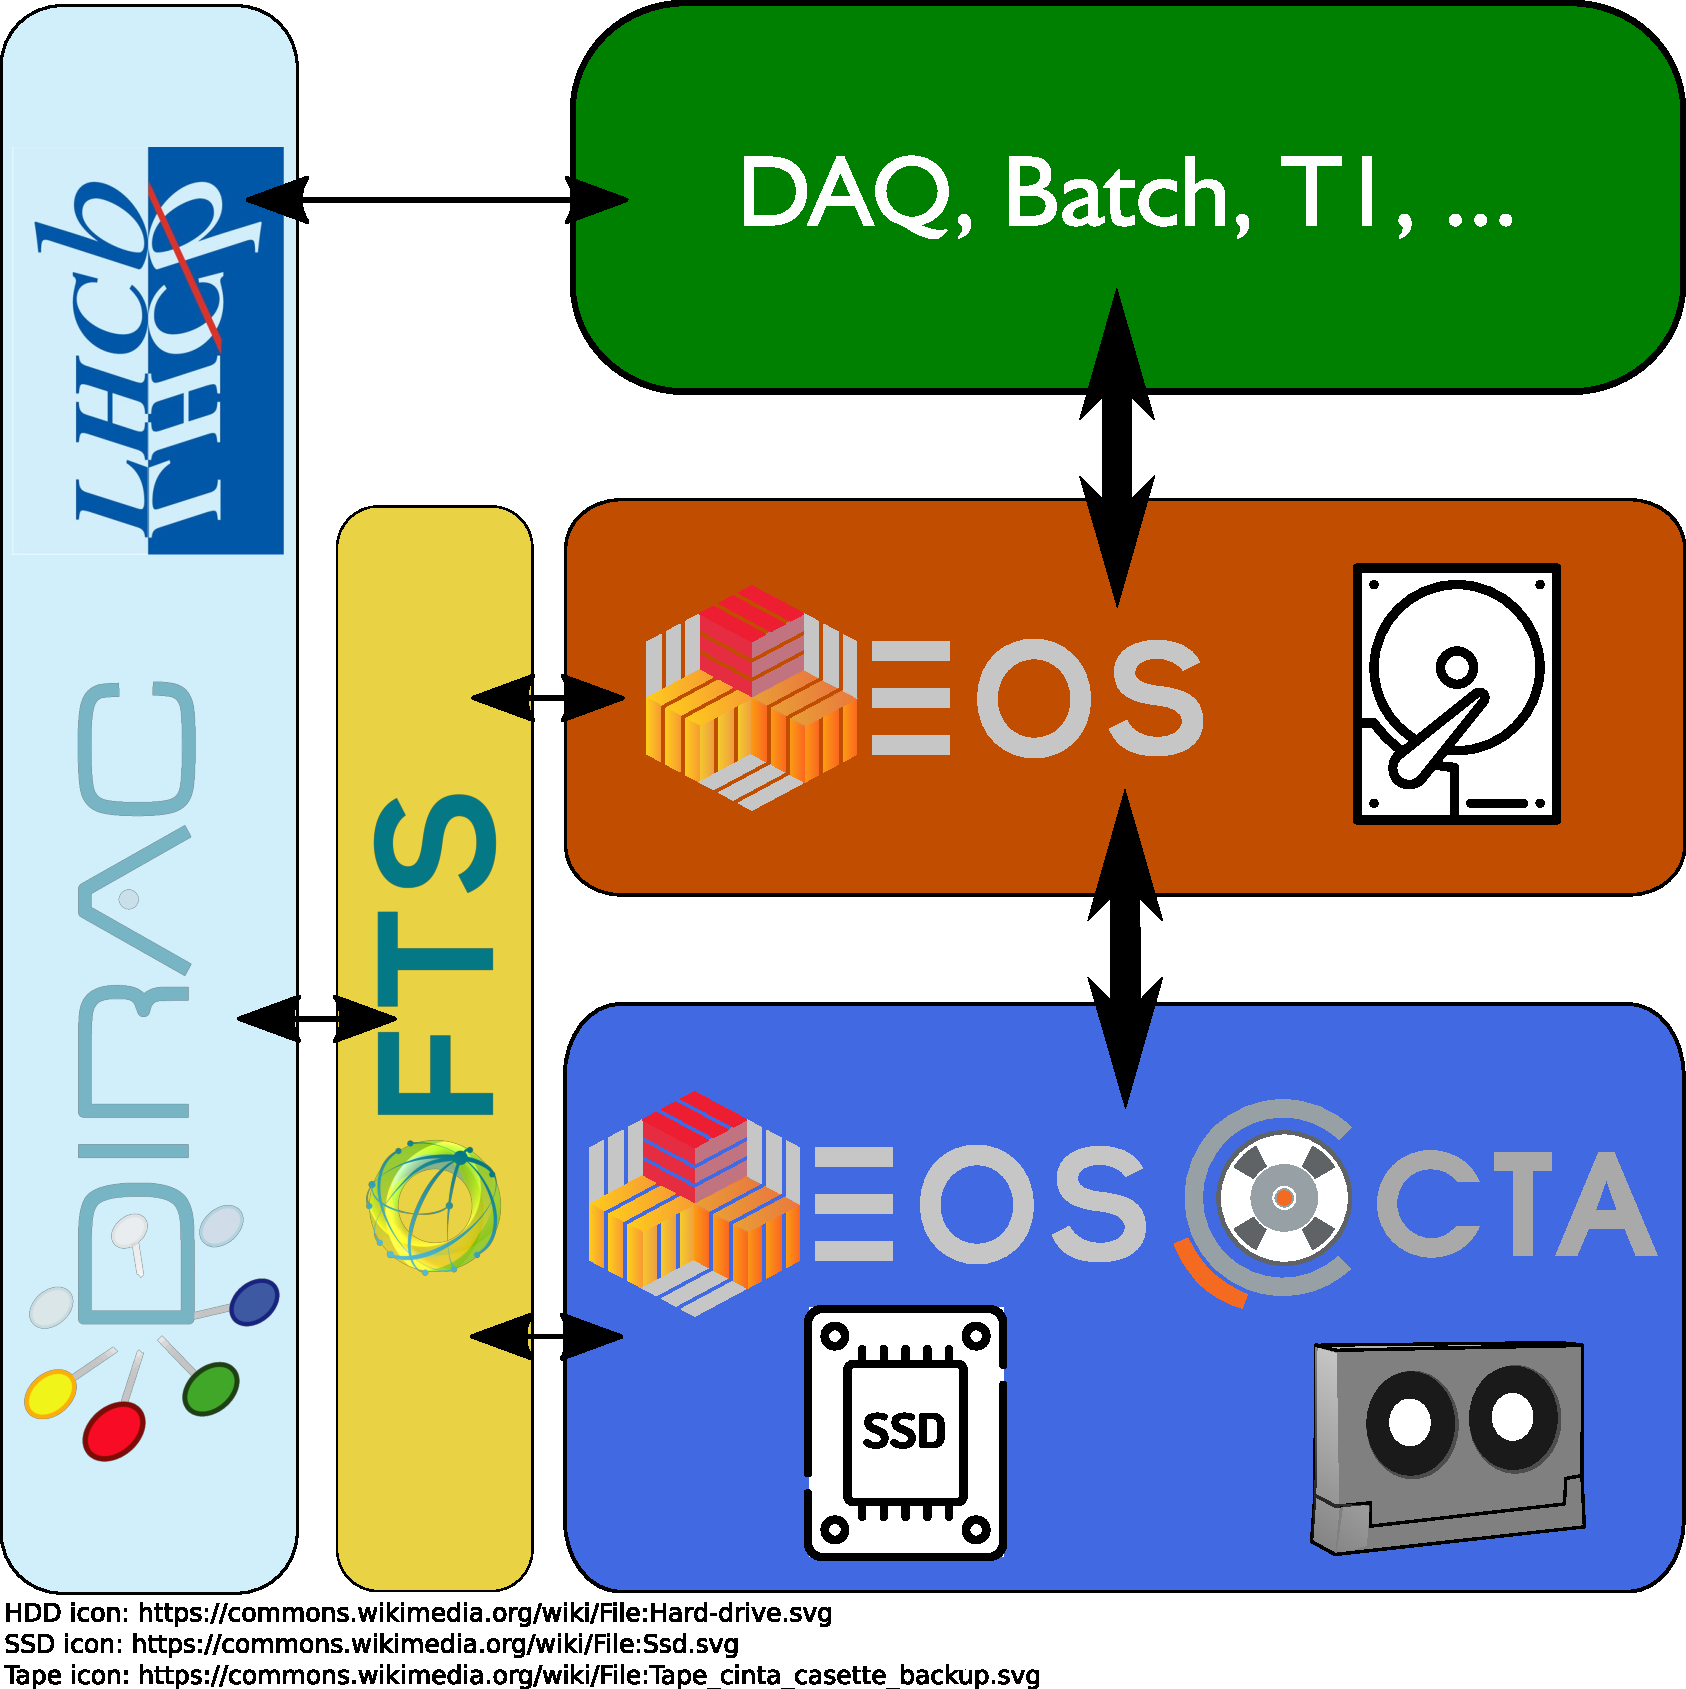
\includegraphics[width=\textwidth]{images/CTA_Deployment_LHCb.pdf}
		\end{center}
	\end{column}
\end{columns}
\end{frame}

\begin{frame}{What's next for CTA?\\
   Non-LHC Experiments}
\begin{columns}
	\begin{column}{0.4\textwidth}
		\begin{center}
		  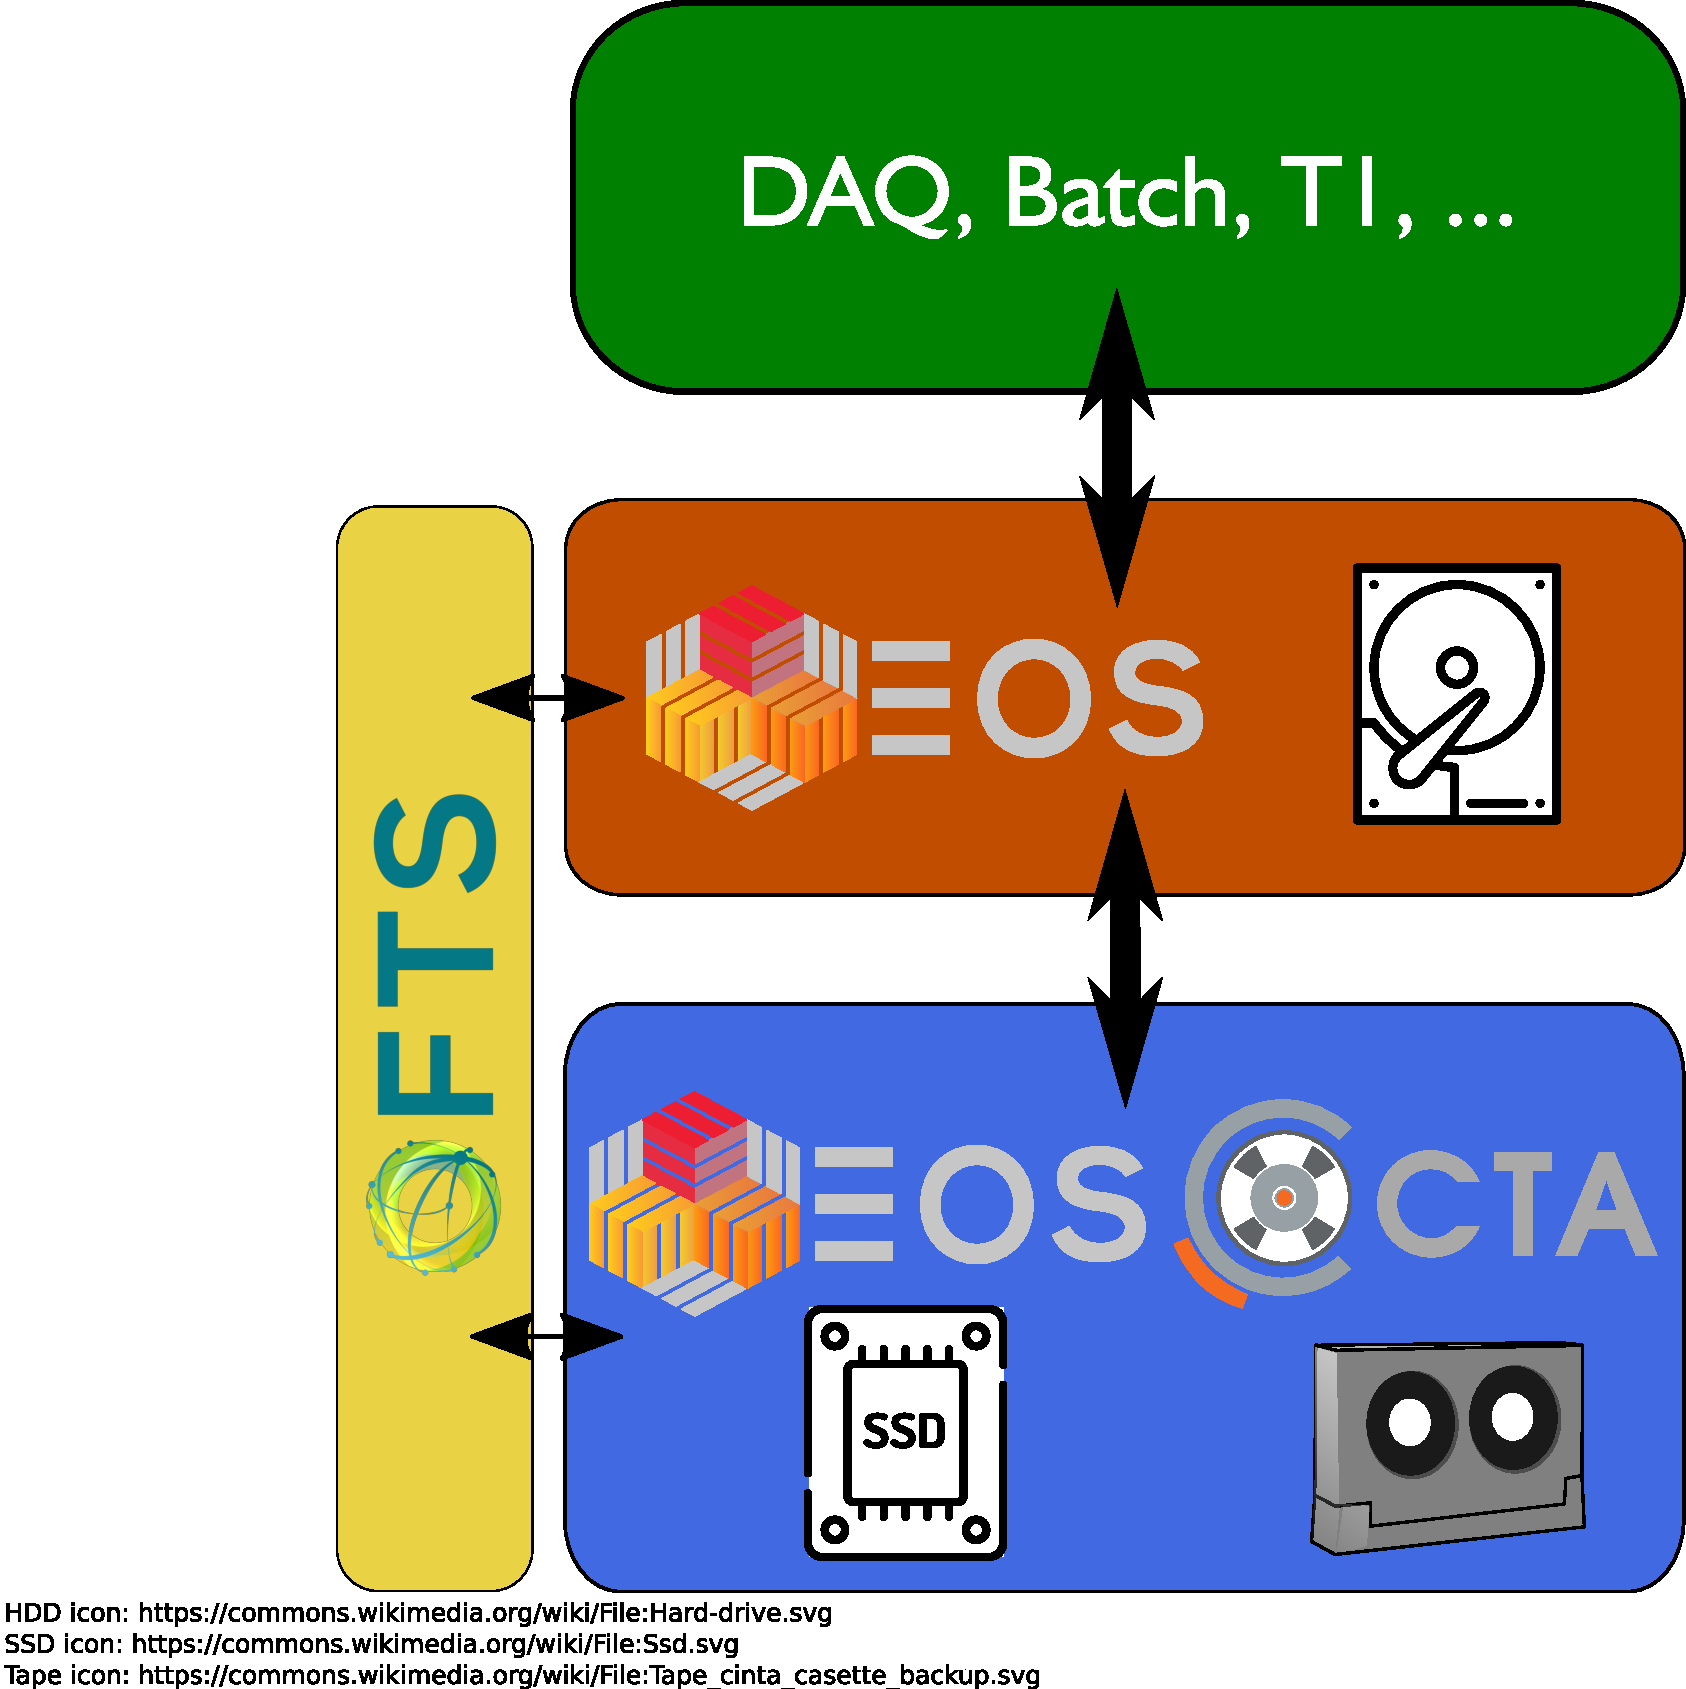
\includegraphics[width=\textwidth]{images/CTA_Deployment_small}
		\end{center}
	\end{column}
	\begin{column}{0.55\textwidth}
      \begin{itemize}
      \item AMS, Compass, Dune, NA61, NA62, nTOF, \ldots
      \item Fellow starting in August: start integration testing with NA62
      \end{itemize}
	\end{column}
\end{columns}
\end{frame}

\begin{frame}{EOS+CTA Status : Summary}{}
\begin{center}

\includegraphics[width=0.5\textwidth]{../Logo/Logo_EOS+CTA}
\end{center}
\begin{itemize}
    \item EOS+CTA ATLAS is in production
    \item CASTOR ATLAS has been retired
    \item ALICE to be migrated in coming months
    \item Integration and commissioning tests for CMS, LHCb and non-LHC experiments
       (schedule to be worked out with each experiment)
\end{itemize}
\end{frame}

\backcover

\end{document}
